\chapter{SNR}

Signal-to-noise ratio (\textit{SNR}) is defined as the relation between a signals power (meaninful information) and its noise power (unwanted information) and its value is normally given in decibel unit.

A continuous-time signals power can be calculated as: 

 \begin{equation}
    P_{signal} = \lim_{T\to\infty} \frac{1}{2T} \int\limits_{-T}^{T} \left |x(t)^2  \right |^2 dt
    \label{Power_eq_cont}
 \end{equation}

Or as:

 \begin{equation}
    P_{signal} = \lim_{N\to\infty} \left ( \frac{1}{2N+1} \sum\limits_{n=-N}^{N} \left |x(n)   \right |^2 dt \right ) 
    \label{Power_eq_disc}
 \end{equation}

for discrete-time signals

Its SNR is:

 \begin{equation}
     SNR = \frac{P_signal}{P_noise}
     \label{SNR_eq}
 \end{equation}

From equation \eqref{SNR_eq} it is possible to know that a higher SNR means a more meaninful signal. To convert this ratio do decibel the following equation is used:

\begin{equation}
    SNR_{dB} = 10log_{10} \left( \frac{P_{signal}}{P_{noise}} \right)
\end{equation}

In the present work there are three ways to estimate the SNR. The first approach is to denoise the raw signal with a filter and then use this denoised signal to obtain the noise one. The main difficulty is to design the proper analog filter, because the denoised signal ideally should have the same magnitude and no phase shift on any signal frequency, however that would require some sort of special filter. To simplify that, a first order filter will be used and its cutoff frequency was choosen after defining the frequency components of a gait as depicted in \ref{fig:FFT_steps}.

\begin{figure}[h]
    \centering
    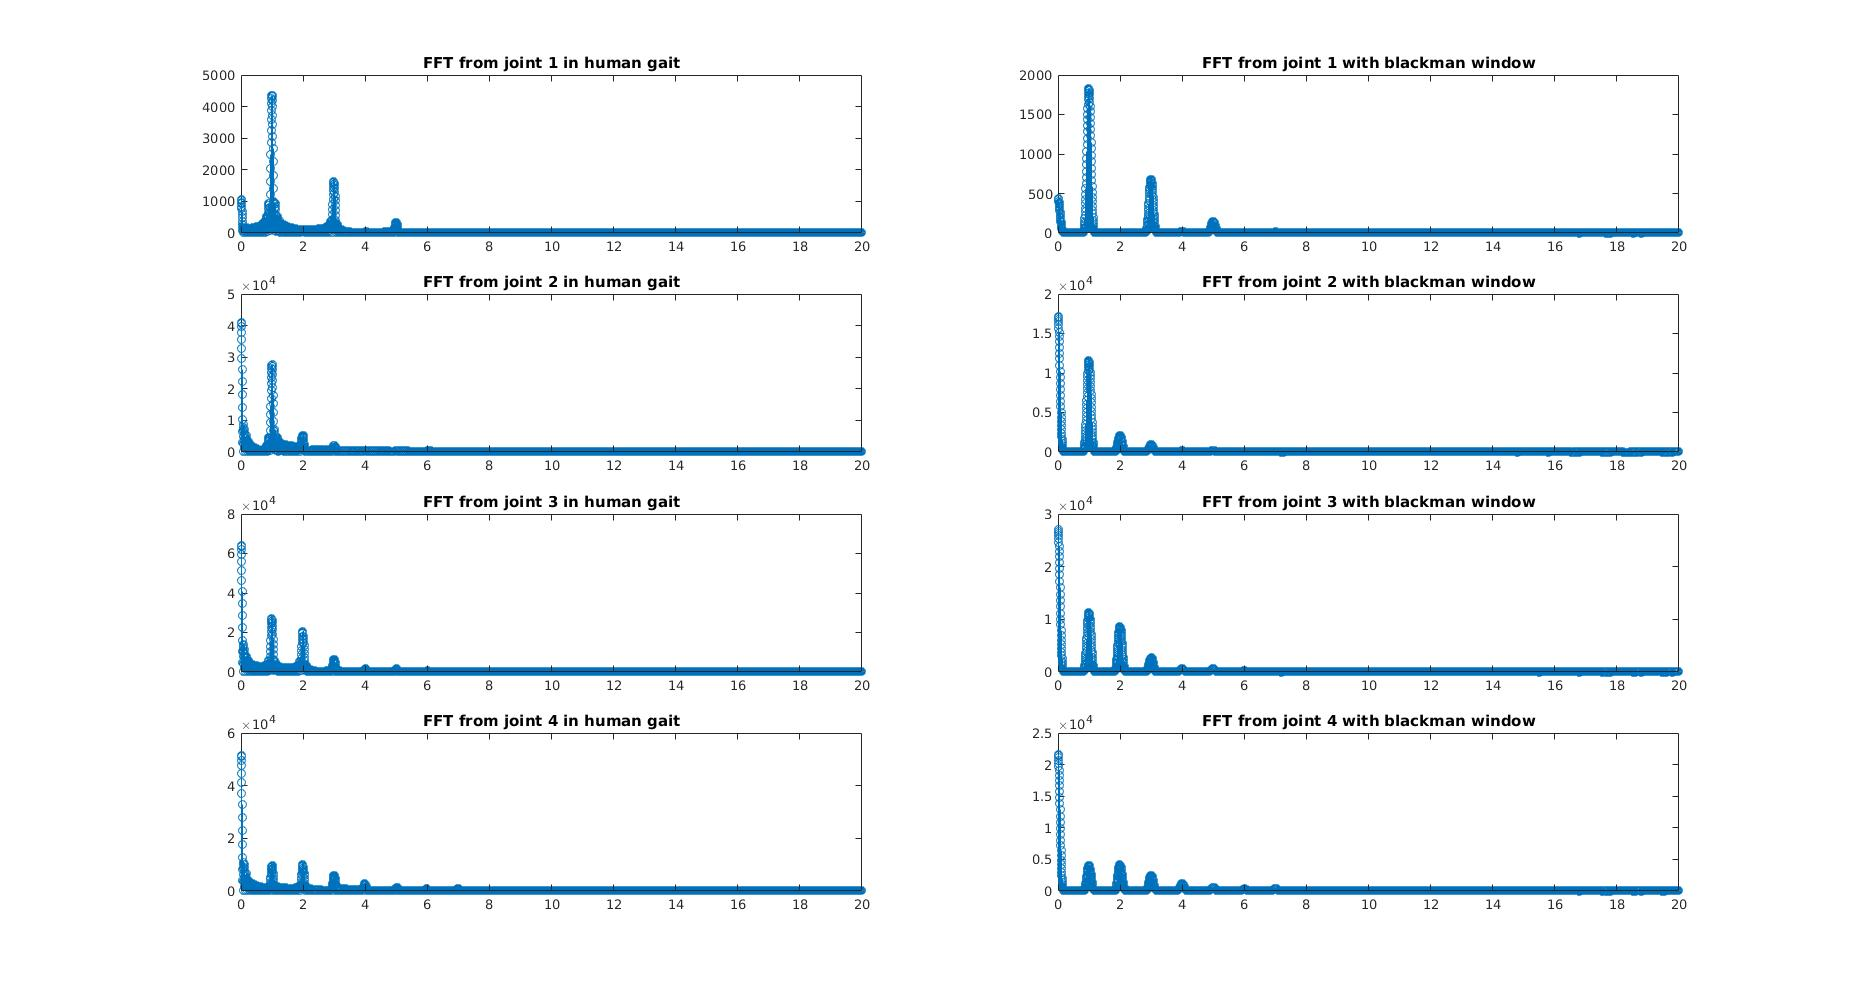
\includegraphics[width=\linewidth]{1sec_step_FFT.jpg}
    \caption{FFT example for Human gait considering a 1 sec step}
    \label{fig:FFT_step}
\end{figure}

